\section{Datasets}
%\textit{In this section the available data sets must be presented. The term dataset refers to any type of information source, for example web services for geolocation fall into this category.}
%\textit{In addition, all necessary data manipulation processes, such as cleaning and enrichment with external sources, must be presented and discussed.}




Il dataset scelto per il nostro progetto \textit{Costa Rican Household Poverty Level Prediction} è reperibile su Kaggle \cite{kaggleCostaRican} e contiene tutte le informazioni relative ad un campione di famiglie che vivono in Costa Rica. Il numero di record che compongono il dataset è 9557 e gli attributi sono 143: ogni record rappresenta una singola persona appartenente ad una determinata famiglia.
La variabile target, che si vuole predire, rappresenta il livello di ricchezza/povertà della famiglia di appartenenza dei vari individui, mentre le altre colonne contengono informazioni riguardanti l'individuo o la sua famiglia.
Sul dataset è stato eseguito un importante preprocessing al fine di analizzare e gestire i missing values e di capire il significato, la distribuzione e l'eventuale utilità dei numerosi attributi presenti, spesso denominati in spagnolo. 

\subsection{Metodi Implementati per l'Analisi delle Variabili}
%[inserire le varie immagini]\\
Durante l'analisi sono stati implementati vari metodi per analizzare e visualizzare la distribuzione delle singole variabili. 
Il metodo \texttt{num\_variable()} viene applicato per l'analisi delle variabili con valori numerici, anche ordinali. Nel caso si rivelasse necessario, il metodo procede a cambiare il nome della variabile ed esegue un'analisi: conta le occorrenze per ogni classe o esegue una descrizione statistica. Infine, riporta il numero di missing values riscontrati. 
Il metodo \texttt{plot\_num\_variable()} viene utilizzato per visualizzare graficamente la distribuzione di una variabile numerica o ordinale. In particolare, i parametri \texttt{many\_values} e \texttt{nonzero} permettono di adattare il grafico alle esigenze della singola variabile.
%\texttt{many\_values == True} viene utilizzata quando si hanno molti valori sull'asse x, mentre \texttt{nonzero == True} quando nessun record assume il valore 0. 
Il metodo \texttt{single\_column()} è stato implementato per passare da una rappresentazione one hot encode di più colonne a una singola colonna contenente come valori i nomi delle singole colonne. 
Il metodo \texttt{cat\_variable()} viene impiegato nelle variabili categoriche (binarie o con stringhe come valori). Effettua se necessario due operazioni: rinomina le colonne e raggruppa più colonne in una singola colonna. Riporta poi il numero di missing values e il conteggio delle occorrenze per ogni classe.
Da ultimo, il metodo \texttt{plot\_cat\_variable()} serve per visualizzare la distribuzione di una variabile binaria o con stringhe come valori. I parametri \texttt{binary} e \texttt{central} sono adoperati per adattare meglio il grafico alla variabile.
%Il parametro \texttt{binary} serve a distinguere questi due casi e utilizzare il giusto grafico, mentre il parametro \texttt{central} è adoperato per avere una migliore leggibilità del grafico.

\subsection{Le Variabili del Dataset}

La variabile \texttt{idhogar} (rinominata \texttt{id\_family}), che riporta gli identificativi di 2988 famiglie, permette di capire la distribuzione del numero di componenti per ogni famiglia (solitamente 2-4).
\texttt{id\_family} e la variabile \texttt{Id}, rappresentante l'identificativo delle singole persone, verranno in seguito rimosse.

%Questa variabile verrà rimossa in quanto non sarà possibile mantenerla né tramite One Hot Encode (determinerebbe la creazione di quasi 3000 colonne), né trasformandola in una variabile numerica (assumerebbe erroneamente le caratteristiche di una variabile ordinale).

%Viene rimossa anche \texttt{Id}, rappresentante l'identificativo delle singole persone.

\subsubsection{Variabili Numeriche}

La variabile \texttt{v2a1} (\texttt{monthly\_rent\_payment}) rappresenta l' ammontare dell'af-fitto mensile di ogni famiglia.
Data l'elevata presenza di missing values (circa 7000) e  un confronto con un'altra variabile \texttt{type\_of\_contract} per cercare di ricavare il maggior numero possibile di valori mancanti, questa variabile è stata rimossa dal dataset. Le successive riportano valori nuemrici ma ordinali.
La variabile \texttt{age} riporta l'età di ogni persona nel dataset, concentrate  tra gli 0 e i 60 anni.
La variabile \texttt{escolari} (\texttt{education\_years}) riporta gli anni di istruzione per ogni persona (la cui moda è 6 anni). 
Dal dataset sono state rimosse le variabili \texttt{rez\_esc}, numero di anni scolastici indietro per ogni persona, che contiene un altissimo numero di missing values, e \texttt{meaneduc}, numero medio di anni di istruzione degli adulti della famiglia, informazione ricavabile dalle altre variabili.
Le variabili \texttt{hogar\_nin} (\texttt{num\_child-} \texttt{ren}), \texttt{hogar\_adult} (\texttt{num\_adults}) e  \texttt{hogar\_mayor} (\texttt{num\_enderly}) rappresentano rispettivamente il numero di bambini (età inferiore a 19 anni), adulti e anziani (età superiore a 65 anni) presenti in ogni famiglia. Mediamente, le famiglie sono composte da 1/2 bambini, 2/3 adulti e 0 anziani.
Dalla combinazione di queste variabili è possibile ricavare il numero totale di persone presenti all'interno della famiglia, rendendo superflue le variabili \texttt{r4t3}, \texttt{tamhog}, \texttt{tamviv}, \texttt{hhsize} e \texttt{hogar\_total}. Infine, viene eliminata anche \texttt{dependecy}, che riporta il rapporto tra il numero di bambini o anziani e il numero di adulti per famiglia. 
Le variabili \texttt{rooms} e \texttt{bedrooms} indicano rispettivamente il numero di stanze e camere da letto presenti nelle case di ogni famiglia.
Le informazioni riportate da queste variabili congiunte con il numero di persone in ogni famiglia rendono superflue le variabili: \texttt{overcrowding}, numero di persone per stanza, \texttt{hacdor}, presenza di sovraffollamento riferito al numero di camere da letto e \texttt{hacapo}, presenza di sovraffollamento riferito al numero di stanze.
Le variabili \texttt{r4m3} (\texttt{tot\_females}) e \texttt{r4h3} (\texttt{tot\_males}) riportano rispettivamente il numero di donne e uomini all'interno della famiglia (mediamente due femmine e due maschi).
Vengono quindi rimosse alcune variabili ottenute combinando informazioni riguardanti genere e età dei componenti della famiglia (\texttt{r4h1}, \texttt{r4h2}, \texttt{r4m1}, \texttt{r4m2}, \texttt{r4t1}, \texttt{r4t2}).
La variabile \texttt{hv18q1} (\texttt{num\_tablets}) riporta il numero di tablet per ogni famiglia, riconducibili all'assenza degli stessi e pertanto sotituiti con il valore 0.
La variabile \texttt{qmobilephone} (\texttt{num\_phones}) riporta il numero di telefoni presenti nella famiglia, mediamente 2/3 a famiglia.
Le variabili \texttt{edjefe} e \texttt{edjefa} (unite in \texttt{household\_head\_education}) riportano gli anni di istruzione del capo famiglia. Esse contenevano, oltre a valori numerici, anche i valori \textit{yes} e \textit{no}, sostituiti con i valori numerici 1 e 0.

\subsubsection{Variabili Binarie}

La variabile \texttt{v14a} (\texttt{has\_bathroom}) e  \texttt{refrig} (\texttt{has\_refrigerator}) indicano rispettivamente la presenza o assenza del bagno e del frigorifero all'interno della casa della famiglia.
Le variabili \texttt{v18q} (\texttt{has\_tablet}), \texttt{mobilphone} (\texttt{has \_phone}), \texttt{computer} (\texttt{has\_computer}),  \texttt{television} (\texttt{has\_television}), indicano se la famiglia dell' individuo considerato possiede o meno tablet, computer, televisione e telefono.
La maggior parte delle famiglie non dispongono di questi dispositivi, ad eccezione del telefono.
La variabile \texttt{cielorazo} (\texttt{has\_ceiling}) indica la presenza o assenza del soffitto nella casa.
La variabile \texttt{dis} (\texttt{is\_disabled}) indica se l'individuo considerato è disabile.

\subsubsection{Variabili Categoriche}

Le variabili \texttt{female} e \texttt{male} (unite in \texttt{gender}) rappresentano il genere dell'indi-viduo, la cui quantità nel campione è bilanciata.
Le 7 variabili \texttt{estadocivl} (unite in \texttt{marital\_status}) riportano lo stato civile dell'individuo considerato (in maggioranza single e sposati).
Le 12 variabili \texttt{parentesco} (aggregate in \texttt{relationship}) riportano il grado di parentela che lega ogni individuo al capofamiglia (in maggioranza figli del capofamiglia). Le 9 variabili \texttt{instlevel} (unite in \texttt{education}) rappresentano il tipo di istruzione conseguita da ogni persona.
Le 8 variabili \texttt{pared} (unite in \texttt{outside\_wall}), le 6 \texttt{piso} (unite in \texttt{floor}) e le 4 \texttt{techo} (unite in \texttt{roof}) riguardano il materiale con cui sono fatte rispettivamente le pareti, il pavimento e il tetto dell'abitazione dell'individuo. 
Le 3 variabili \texttt{abastagua} (aggregate in \texttt{water\_provision}), le variabili \texttt{public}, \texttt{planpri}, \texttt{noelec} e \texttt{coopele} (unite in \texttt{electricity\_source}), le 5 variabili \texttt{sanitario} (unite in \texttt{toilet\_system}), le 4 \texttt{energcocinar} (unite in \texttt{energy}) e le 6 \texttt{elimbasu} (unite in \texttt{rubbish\_disposal}) riportano rispettivamente la tipologia di: approvvigionamento dell'acqua, di impianto elettrico, di sistema di servizi igienici, di cucina e di sistema smaltimento dei rifiuti. 
Le 3 variabili \texttt{etecho} (unite in \texttt{roof} \texttt{status}), le 3 \texttt{eviv} (unite in \texttt{floor} \texttt{status}) e le 3 \texttt{epared} (unite in \texttt{walls\_status}), indicano rispettivamente lo stato del tetto, del pavimento e delle pareti dell'abitazione.
Le 5 variabili \texttt{tipoviv} (aggregate in \texttt{type\_of\_contract}) indicano la tipologia di contratto che la famiglia ha stipulato per la casa. La maggioranza sono case di proprietà, seguite da quelle affittate. 
Le 6 variabili \texttt{lugar} (unite in \texttt{region}) e le 2 \texttt{area} rappresentano rispettivamente la regione e l'area in cui risiede l'individuo. 

\subsubsection{Variabile Target}
La variabile \texttt{target} (Figura \ref{fig:distrTarget}) riporta il grado di povertà/ricchezza, e quindi di vulnerabilità, della famiglia dell'individuo. 
Essa può assumere i valori: 1 - povertà estrema, 2 - povertà moderata, 3 - famiglia vulnerabile e 4 - famiglia non vulnerabile.
Il 63\% degli individui appartiene a famiglie non vulnerabili, determinando un dataset un po' sbilanciato.

\begin{figure}[H]
     \centering
     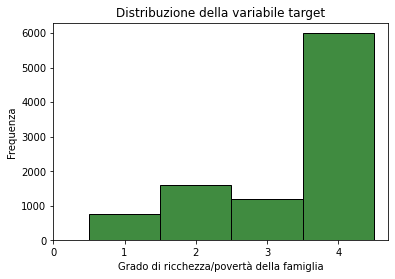
\includegraphics[scale=0.5]{Latex template for Project Report-20220108/immagini/distribuzione target.png}
     \caption{Distribuzione della variabile target}
     \label{fig:distrTarget}
\end{figure}

